\documentclass[12pt]{article}

\usepackage{sbc-template}
\usepackage{graphicx,url}
\usepackage[utf8]{inputenc}
\usepackage[brazil]{babel}
%\usepackage[latin1]{inputenc}  
\usepackage{setspace}
\usepackage{amsmath}
\usepackage{algorithm}
\usepackage[noend]{algpseudocode}     
\usepackage{listings}
\usepackage{xcolor}
\lstset { %
    language=C++,
    backgroundcolor=\color{black!5}, % set backgroundcolor
    basicstyle=\footnotesize,% basic font setting
}


\sloppy
\title{Processamento Digital de Imagens em Plataformas Embarcadas}

\author{Erick Modesto Campos}


\address{Instituto de Ciência Exatas e Naturais (ICEN) -- Universidade Federal do Pará
  (UFPA)\\
  Laboratório de Visualização, Interação e Sistemas Inteligentes (LabVis - UFPA)\\
  Cep 66075110 -- Guamá-- Belém -- Pará -- Brazil
  \email{erick.c.modesto@gmail.com / erickcampos@ufpa.br}
}


\begin{document} 

\onehalfspace
\maketitle

\begin{abstract}
Image processing is a method that performs a series of mathematical operations
on an image. The intent is to get an enhancement or extract some useful
information about the image being processed. Although image processing
algorithms generally run on more robust machines, it is also possible to employ
these tasks on embedded systems. In this sense, this work aims to use the
Raspberry Pi platform, more specifically the Raspberry Pi 3 model B version. The
idea is to apply grayscale conversion algorithms on low cost platforms that have
a multicore architecture to be able to perform parallelism techniques, making
the most of the processing power of the platform used.
\end{abstract}
     
\begin{resumo} 
O processamento de imagens é um método que executa uma série de operações
matemáticas em uma imagem.  intuito é obter um aprimoramento ou extrair algumas
informações úteis a cerca da imagem a ser processada. Apesar dos algoritmos de
processamento de imagens serem executados geralmente em máquinas mais robustas,
é possível também empregar essas tarefas em sistemas embarcados.  Nesse sentido,
este trabalho tem como proposta utilizar a plataforma Raspberry Pi, mais
espicificamente a versão Raspberry Pi 3 modelo B. A ideia é aplicar algoritmos
de conversão em escala de cinza em plataformas de baixo custo e que possuem uma
arquitetura multicore para que seja capaz de aplicar tecnicas de paralelismo,
aproveitando ao máximo o poder de processamento da plataforma utilizada.
\end{resumo}

\begin{section}{Introdução}
O processamento de imagens é um método que executa uma série de operações
matemáticas em uma imagem. O intuito é obter um aprimoramento ou extrair algumas
informações úteis a cerca da imagem a ser processada. Esse método nada mais é do
que um processamento digital de sinais onde a entrada é uma imagem e a saída
pode ser uma imagem ou características (\textit{features}) associadas com a
determinada imagem processada~\cite{Tartu19}.

A área de processamento de imagens existem diversos algoritmos que são
utilizados para diversos propósitos. O reconhocimento de objetos é um bom
exemplo de aplicação das técnicas de processamento. No entanto, assim como
outros algoritmos, é necessário realizar várias aplicações chamadas de
pré-processamento. E geralmente os sistemas que implementam o reconhecimento de
objetos em uma imagem, utilizam conversão da imagem original para a escala de
cinza como primeira etapa de pré-processamento.

\end{section}
\begin{section}{Trabalhos Relacionados}
Pipeline é uma técnica bem antiga e bastante conhecida por ser empregada na
linha de produção industrial. A ideia por trás dessa técnica é bastante simples.
Um processo passa por vários estágios da linha de montagem, subdividindo em
tarefas menores, e essa linha de montagem é continuamente alimentada de novos
processos. Em cada estágio uma parte de um processo é finalizado e passado para
o próximo estágio. Quando é chegado no ultimo estágio, cada subprocesso
finalizado é reunido e então finalmente finalizado
completamente~\cite{Bhujade95}. Um bom exemplo da aplicação dessa técnica é na
industria automobilística onde são construídos diversos carros simultaneamente.
A Figura~\ref{fig:carro} mostra a ilustração da aplicação do pipeline na linha
de montagem de um carro.

\begin{figure}[!h]
	\centering
	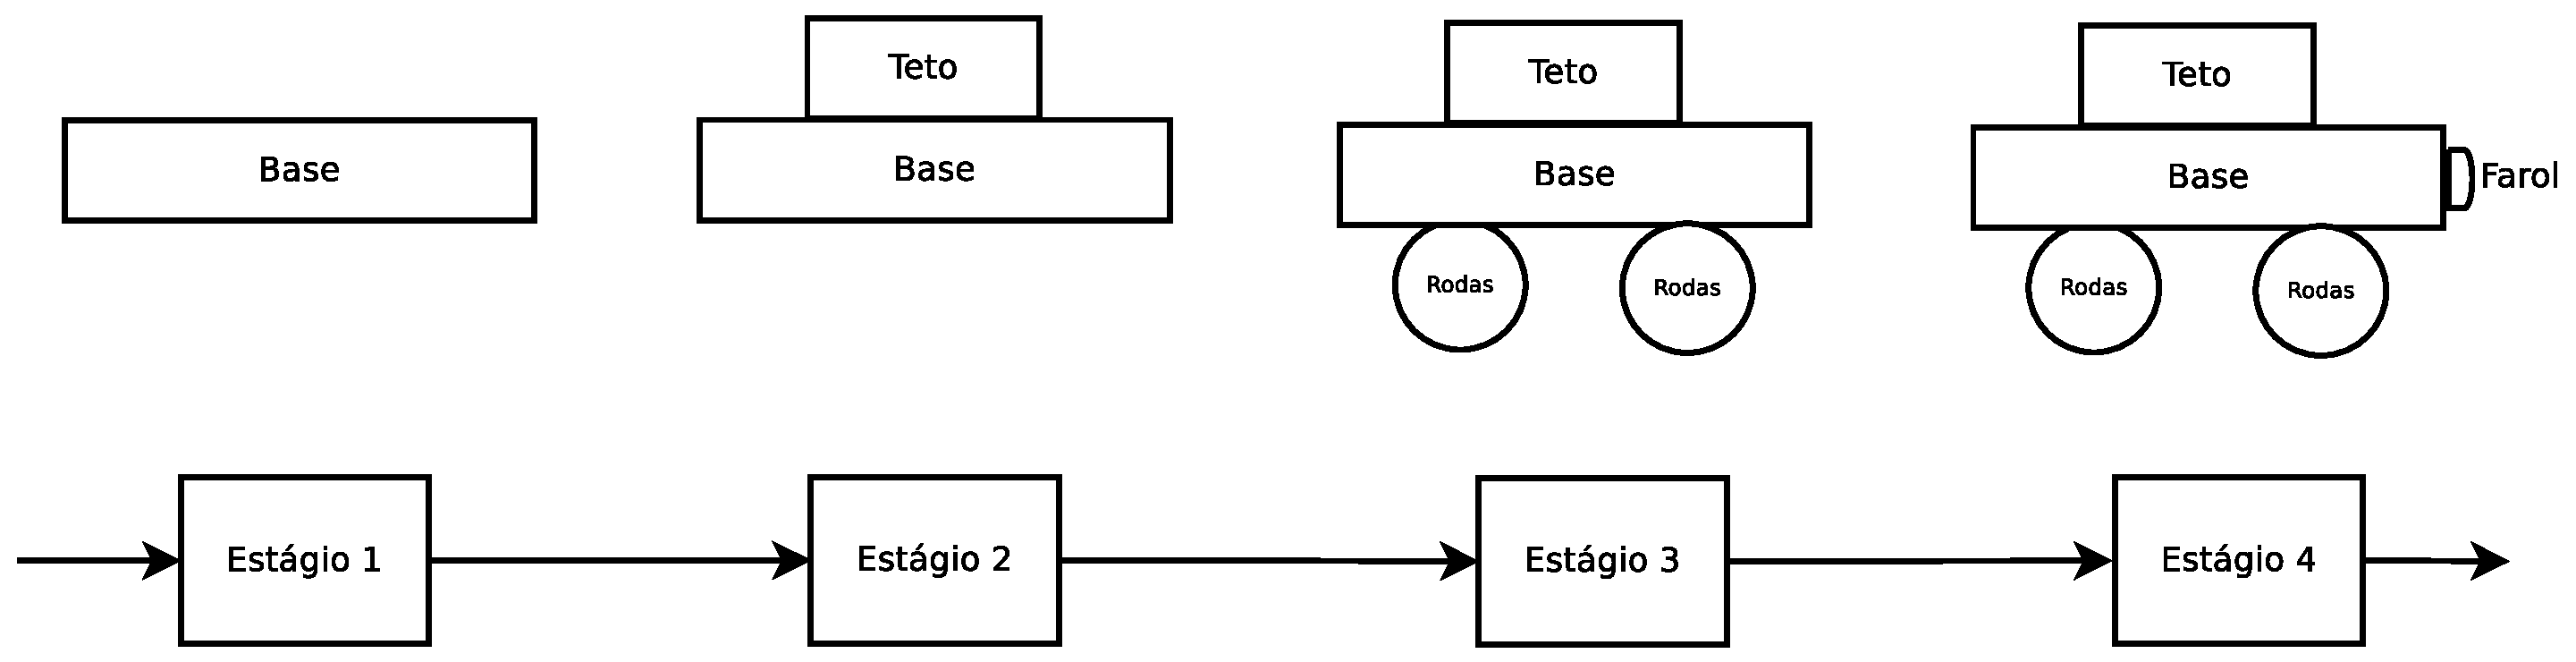
\includegraphics[width=0.95\linewidth]{figs/carro}
	\caption{Processo de uma linha de montagem da industria automobilística.}
	\label{fig:carro}
\end{figure}

Na computação essa técnica foi também incorporada para o desenvolvimento de
programas. Com a grande variedade de processadores multicore, houve a
necessidade de aproveitar ao máximo o poder de processamento de cada núcleo do
processador. A execução de tarefas sequenciais não é a melhor forma de obter
alto desempenho de processamento. Nesse sentido, o pipelining se torna uma
técnica alternativa para aumentar o desempenho de tarefas sequenciais de
\textit{software}.

Ao utilizar a técnica de pipelining, um processo que normalmente seria
executado de forma sequencial é dividido em estágios distintos que podem ser
executados em um modelo de linha de montagem semelhante ao exemplo mostrado
anteriormente, onde dada núcleo do processador fica encarregado de executar uma
subtarefa. 

Dessa forma, o pipelining melhora o desempenho, pois a subdivisão de uma tarefa
em tarefas menores executadas cada uma por um certo processador é mais rápido
para ser finalizada que se cada uma das subtarefas fossem executadas apenas por
um único processador.

É importante ressaltar que para haver uma melhora significativa no desempenho, é
sempre recomendável manter o balanceamento das subtarefas. A
Figura~\ref{fig:bal} mostra a questão do balanceamento.

\begin{figure}[!h]
	\centering
	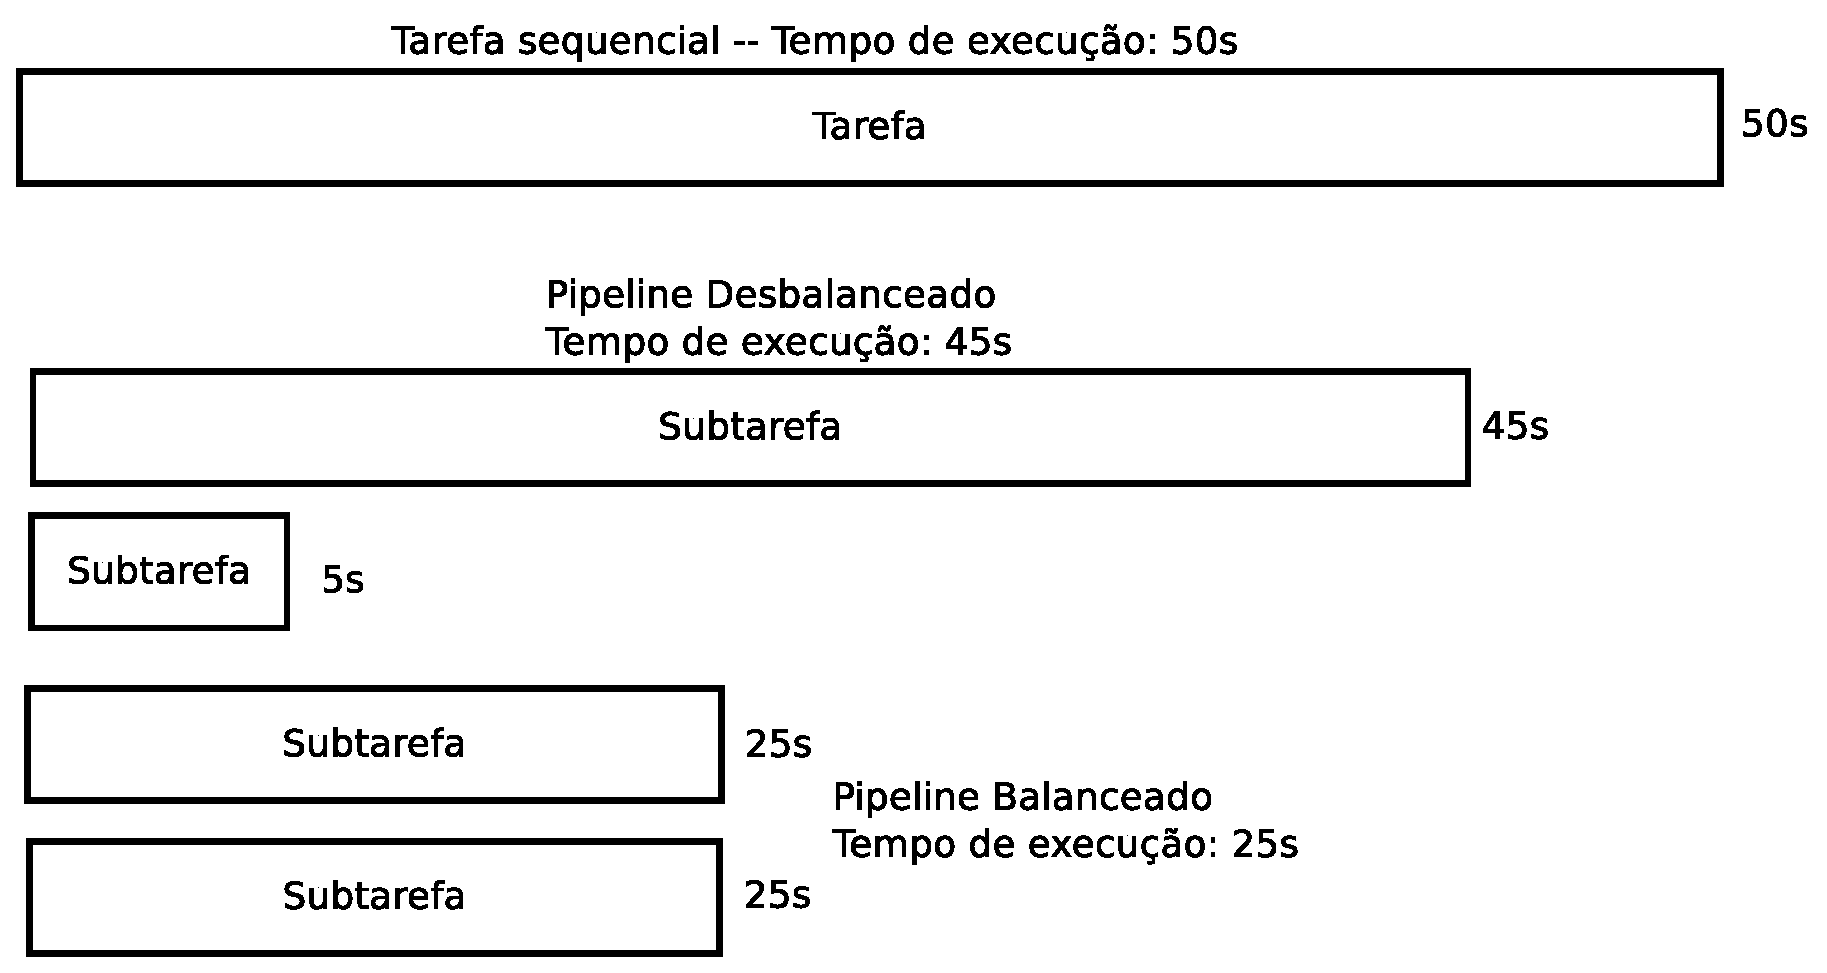
\includegraphics[width=0.95\linewidth]{figs/pipe}
	\caption{Balanceamento de subtarefas.}
	\label{fig:bal}
\end{figure}

O primeiro caso da Figura~\ref{fig:bal} mostra o tempo de execução de uma tarefa
sequencial. Aplicando técnica de pipelining sem levar em conta a questão do
balanceamento, como mostra o segundo caso, o tempo para executar tarefa reduz
pouco se levarmos em conta o tempo da tarefa sequencial. Contudo, se o pipeling
for aplicado com as subtarefas balanceados, o desempenho de execução melhora
consideravelmente, sendo justificável a aplicação dessa técnica para este caso,
visto que o tempo de execução é reduzido pela metade.

\end{section}
\begin{section}{Objetivos}
Esta seção tem como objetivo mostrar a metodogia para implementação do trabalho
proposto.

\begin{subsection}{Forma Sequencial Implementada}


\begin{figure}[!h]
	\centering
	\includegraphics[width=0.95\linewidth]{figs/Sequential.png}
	\caption{Forma sequencial do algoritmo.}
	\label{fig:gray}
\end{figure}



A maioria das imagens digitais é composta por três canais de cores separados: um
canal vermelho, um canal verde e um canal azul. A sobreposição desses canais em
camadas cria uma imagem colorida. Modelos de cores diferentes têm canais
diferentes (às vezes os canais são cores, às vezes são outros valores como
luminosidade ou saturação), mas este trabalho se concentra apenas no RGB.

Todos os algoritmos de conversão do canal RGB para escala de cinza utilizam 
o mesmo processo básico que consistem em três etapas:

\begin{itemize}
\item Obter os valores dos canais vermelho, verde e azul de um \textit{pixel}.
\item Relacionar esses valores para transformar em apenas um valor.
\item Substituir os valores originais de vermelho, verde e azul pelo valor calculado
\end{itemize}


\begin{lstlisting}
for each pixel na imagem{

	vermelho = pixel.Red()
	verde = pixel.Green()
	azul = pizel.Blue()

	Obter_Valor_Cinza = cinza

	pixel.Red = cinza
	pixel.Green = cinza
	pixel.Blue = cinza

}
\end{lstlisting}

Os métodos para obtenção do valor cinza para cada algorimo são apresentados a
seguir.


\begin{figure}[!h]
	\centering
	\includegraphics[width=0.95\linewidth]{figs/gray.png}
	\caption{Resultado dos algoritmos.}
	\label{fig:gray}
\end{figure}

\subsubsection{Algoritmo 1: Média}
O algoritmo baseado na média é a rotina de conversão mais comum em escala de
cinza e o calculo do valor de cinza é obtido a partir da Equação~\ref{eq:media}.

\begin{equation}
\label{eq:media}
cinza = (vermelho + verde + azul)/3
\end{equation}

Essa fórmula gera um equivalente em escala de cinza razoavelmente boa e sua
simplicidade facilita a implementação e otimização. No entanto, esse método não
deixa de ter falhas --- embora rápida e simples, ela faz um mau trabalho em
representar tons de cinza em relação à maneira como os seres humanos percebem a
luminosidade (brilho).


\subsubsection{Algoritmo 2: Luminância}
Esse segundo algoritmo mostra que a densidade do cone no olho humano não é
uniforme entre as cores. Os seres humanos percebem o verde mais fortemente que o
vermelho e o vermelho mais fortemente que o azul. Isso faz sentido do ponto de
vista da biologia evolucionária --- grande parte do mundo natural aparece em
tons de verde, de modo que os humanos desenvolveram maior sensibilidade à luz
verde.

Como os humanos não percebem todas as cores da mesma forma, o ``método da média'' de
conversão em escala de cinza é impreciso. Em vez de tratar as luzes vermelha,
verde e azul igualmente, uma boa conversão em escala de cinza pondera cada cor
com base na maneira como o olho humano a percebe. Uma fórmula comum em
processadores de imagem (Photoshop, GIMP) é apresentada na
Equação~\ref{eq:luminancia}.


\begin{equation}
\label{eq:luminancia}
cinza = (0.3*vermelho + 0.59*verde + 0.11*azul)/3
\end{equation}

\subsubsection{Algoritmo 3: Luma}

Assim como no algoritmo 2, este método tenta uniformizar a forma como o ser
humano perceber as cores. Para isso, também é utilizada uma média ponderada
entre os canais como é mostrado na Equação~\ref{eq:luma}

\begin{equation}
\label{eq:luma}
cinza = (0.2126*vermelho + 0.7152*verde + 0.0722*azul)/3
\end{equation}


\subsubsection{Algoritmo 4: Dessaturação}

A maioria dos programadores usa o modelo de cores RGB. Embora seja uma boa
maneira de uma máquina descrever cores, o espaço de cores RGB pode ser difícil
para a percepção humana. Nesse sentido, o espaço de color HSL (do inglês
\textit{hue, saturation, lightness}) é algumas vezes utilizado para a
vizualização das cores. A matiz (\textit{Hue}) pode ser considerada o nome da
cor --- vermelho, verde, laranja, amarelo etc.  A saturação
(\textit{saturation}) descreve como uma cor é vívida; uma cor muito vívida tem
saturação total, enquanto o cinza não tem saturação. 

A dessaturação de uma imagem funciona convertendo o espaço RGB no espaço HSL e 
forçando a saturação para zero. Um pixel pode ser dessaturado encontrando o
ponto médio entre o máximo de (R, G, B) e o mínimo de (R, G, B), como mostra a
Equação~\ref{eq:dessatura}.

\begin{equation}
\label{eq:dessatura}
cinza = ( Max(vermelho, verde, azul) + Min(vermelho, verde, azul) ) / 2
\end{equation}



\subsubsection{Algoritmo 5: Decomposição}
A decomposição de uma imagem oPde ser considerada uma forma mais simples de
dessaturação. Para decompor uma imagem, cada \textit{pixel} é forçado parao
valor mais alto (máximo) ou mais baixo (mínimo) de seus valores em vermelho,
verde e azul. As Equações~\ref{eq:a} e~\ref{eq:b} mostram como calcular a
decomposição máxima e mínima, respectivamente.

\begin{subequations}

\begin{equation}
\label{eq:a}
cinza = Max(vermelho, verde, azul) 
\end{equation}

\vspace{-1cm}

\begin{equation}
\label{eq:b}
cinza =  Min(vermelho, verde, azul) 
\end{equation}
\end{subequations}


\subsubsection{Algoritmo 6: Canal de cor única}

Este algoritmo representa o método computacional mais simples para conversão em
escala de cinza. Ao contrário de todos os métodos apresentados, este método 
não requer cálculos. Apenas é necessário escolher o valor de um determinado
canal e aplicar para ao valor de cinza, como mostrado na
Equação~\ref{eq:a1},~\ref{eq:b1} e~\ref{eq:c1}

\begin{subequations}

\begin{equation}
\label{eq:a1}
cinza = vermelho 
\end{equation}

\vspace{-1cm}

\begin{equation}
\label{eq:b1}
cinza =  verde 
\end{equation}

\vspace{-1cm}

\begin{equation}
\label{eq:c1}
cinza =  azul 
\end{equation}
\end{subequations}
  
\subsubsection{Algoritmo 7: Tons de cinza}
Este método permite ao usuário especificar quantos tons de cinza a imagem
resultante utilizará. O algoritmo definir o número de tons de cinza da imagem
convertida. Esse método é um pouco mais trabalhoso se comparado com os demais
algoritmos apresentados. Os procedimentos do algoritmo é mostrado a seguir.


\begin{lstlisting}
for each pixel na imagem{
	fator = 255 / (TonsDeCinza - 1)
	metodo = (vermelho + verde + azul)/3
	cinza = (int)((medio / fator) + 0.5) * fator

	//TonsDeCinza: valor entre 2 e 256
}
\end{lstlisting}

\end{subsection}






\end{section}
\begin{section}{Metodologia}
Como descrito, a técnica denominada de pipeline é bastante simples e robusta que
pode ser utilizada em aplicações que demandem melhoria de desempenho na execução
dos processosi. A questão do balanceamneto sempre deve ser levada em
consideração para que o aplicação dessa técnica seja eficaz, contudo nem sempre
é fácil balancear as subtarefas. Portanto, se uma aplicação necessitar ser
executada com um desempenho superior às tarefas seriais, o pipelining pode ser
uma boa alternativa a ser aplicada nesse caso.


\end{section}
\begin{section}{Paralelismo}
Esta seção tem como objetivo mostrar aplicação do paralelismo sobre os
algoritmos analisados neste trabalho.

\subsection{OpenMP}

Para a aplicação do paralelismo utilizando a biblioteca OpenMP, foi utilizada a
abordagem de processar uma imagem por vez, mas subdividindo as imagens em quatro
partes iguais. Um exemplo dessa subdivisão pode ser vista na
Figura~\ref{fig:lena}.

\begin{figure}[!h]
	\centering
	\includegraphics[width=0.3\linewidth]{figs/lenna.png}
	\caption{Subdivisão das imagens.}
	\label{fig:lena}
\end{figure}

Cada processador fica responsável por realizar o algoritmo de conversão em
escala de cinza em uma determinada região da imagem (quando é utilizado
realmente 4 \textit{threads}). Todo esse processo é realizado para cada imagem
até que todas as imagens sejam processadas.

\subsection{OpenMPI}

Já para a aplicação do paralelismo utilizando a biblioteca OpenMPI, foi
realizada a abordagem de processar uma imagem em cada núcleo de processamento.
Dessa forma, blocos de no máximo quatro imagens são carregados de uma vez para o
processamento. A Figura~\ref{fig:mpi} ilustra a aplicação dessa abordagem.

\begin{figure}[!h]
	\centering
	\includegraphics[width=0.5\linewidth]{figs/mpi}
	\caption{Abordagem aplicada.}
	\label{fig:mpi}
\end{figure}

A quantidade de imagens carregadas é igual a quantidade de núcleos de
processamento utilizado. A imagem~\ref{fig:mpi} mostra o carregamento de quatro
imagens de uma vez para ser processadas por quatro núcleos de forma
independente. Esse tipo de abordagem causa um desbalanceamento quando é
executado com três núcles, pois a quantidade de imagens da base não é divisível
por três.





\end{section}
\begin{section}{Avaliação de Desempenho}
Para realizar as simulações, foi determinado cenários diferentes onde cada
cenário executou o código com uma certa quantidade de processadores. Dessa forma
foi possível medir o desempenho conforme a quantidade de processadores
utilizadas. Para cada cenário, o código foi executado cinco vezes e foi coletado
a média dessas cinco execuções para representar o tempo de execução.

Para a análise do desempenho foi utilizado as seguintes métricas:

\begin{itemize}
\item Tempo de execução
\item \textit{Speedup}
\item Eficiência
\item Desempenho
\end{itemize}

O tempo de execução é a soma do tempo de computação, tempo de comunicação e o
tempo ocioso, como mostrado na Equação~\ref{eq:tempo}. 

\begin{equation}
\label{eq:tempo}
T_{exec} = T_{comput} + T_{comunic} + T_{ocioso}
\end{equation}
O \textit{speedup} é a razão entre o tempo de execução em apenas um
processador e o tempo de execução em múltiplos processadores. A
equação~\ref{eq:speedup} mostra o cálculo do \textit{speedup}.

\begin{equation}
\label{eq:speedup}
S = \frac{tempo~1~processador}{tempo~N~processadores}
\end{equation}

A eficiência é determinada pela relação entre o speedup obtido e o
número de processadores necessários para obtê-lo, como mostrado na
Equação~\ref{eq:eficiencia}.

\begin{equation}
\label{eq:eficiencia}
E = \frac{Speedup}{numero~de~processadores}
\end{equation}

Já o desempenho Determina o ``quanto'' os processadores estão sendo
utilizados e é calculado pela Equação~\ref{eq:desempenho}.

\begin{equation}
\label{eq:desempenho}
D = E\times100\%
\end{equation}


\subsection{Desempenho OpenMP}

A Tabela~\ref{tab:analise} mostra o resultados da avaliação de desempenho para o
paralelismo aplicado utilizando a biblioteca OpenMP.

\begin{table}[h]
\centering
\caption{OpenMP: análise de desempenho}
\begin{tabular}{ccccc}
\hline
\textbf{Nº CPU}&\textbf{Tempo exec.}&\textbf{\textit{Speedup}}&\textbf{Eficiência}&\textbf{Desempenho}\\
\hline
1 & 4h8m7s & -- & -- & --  \\
2 & 2h12m38s & 1.870 & 0.935 & 93.5\% \\
3 & 1h39m22s & 2.496 & 0.832 & 83.2\% \\
4 & 1h17m17s & 3.210 & 0.802 & 80.2\% \\ 
\hline
\end{tabular}
\label{tab:analise}
\end{table}

É possível perceber que o tempo de execução diminuiu consideravelmente a medida
que a quantidade de processadores aumentou. Ou seja, a utilização do paralelismo
foi imprescindível para que o tempo de execução melhorasse. Contudo o desempenho
dos processares foi inversamente proporcional, ao número de \textit{threads}
utilizados.

\end{section}
\begin{section}{Considerações Finais}
\input{secs/sec7.tex}
\end{section}

\bibliographystyle{sbc}
\bibliography{sbc-template}

\end{document}
